\documentclass{beamer}
\usetheme{Madrid}
\title[Learned Convex Regularizers]{Learned Convex Regularizers for Inverse Problems}
\subtitle{Mathematical Data Analysis Seminar}
\author{Marko Lalovic}
\date{\today}
\beamertemplatenavigationsymbolsempty

\newcommand{\norm}[1]{\left\lVert#1\right\rVert}
\usepackage{amsmath}
\DeclareMathOperator*{\argmax}{arg\,max}
\DeclareMathOperator*{\argmin}{arg\,min}
\DeclareMathOperator{\EX}{\mathbb{E}}

\usepackage{tikz,tikz-cd}
\usetikzlibrary{calc}
\usetikzlibrary{positioning}
\usetikzlibrary{arrows}

\setbeamertemplate{caption}{\raggedright\insertcaption\par}

\usepackage{bm}
\usefonttheme{professionalfonts}
\usepackage{subcaption}
\usepackage{mathtools}

\begin{document}
\begin{frame}
    \titlepage 
\end{frame}

\begin{frame}{Motivational Examples}
Example: Find solution of $y = Ax$, $A: \mathbb{R}^{n} \rightarrow \mathbb{R}^{m}$, $m < n$
\begin{center}
\begin{figure}
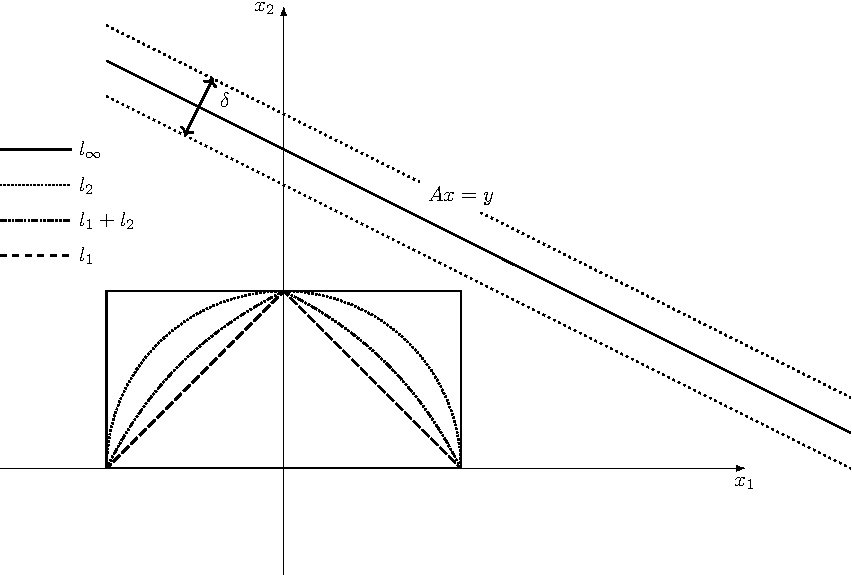
\includegraphics[width=.99\textwidth]{../figures/norms-crop.pdf}
\end{figure}
\end{center}
\end{frame}

\begin{frame}{Motivational Examples - Continued}
Examples:
\begin{itemize}
\item Generate realistic images in HD~\footnote{{\tiny \color{blue} Tero Karras et al.\ ``Progressive Growing of GANs for Improved Quality, Stability, and Variation", arxiv 2018}}
\item Extract main building blocks of images~\footnote{{\tiny \color{blue} Longfei Liu et al. ``X-GANs: Image Reconstruction Made Easy for Extreme Cases", arxiv 2018}}
\end{itemize}
\begin{center}
\begin{figure}
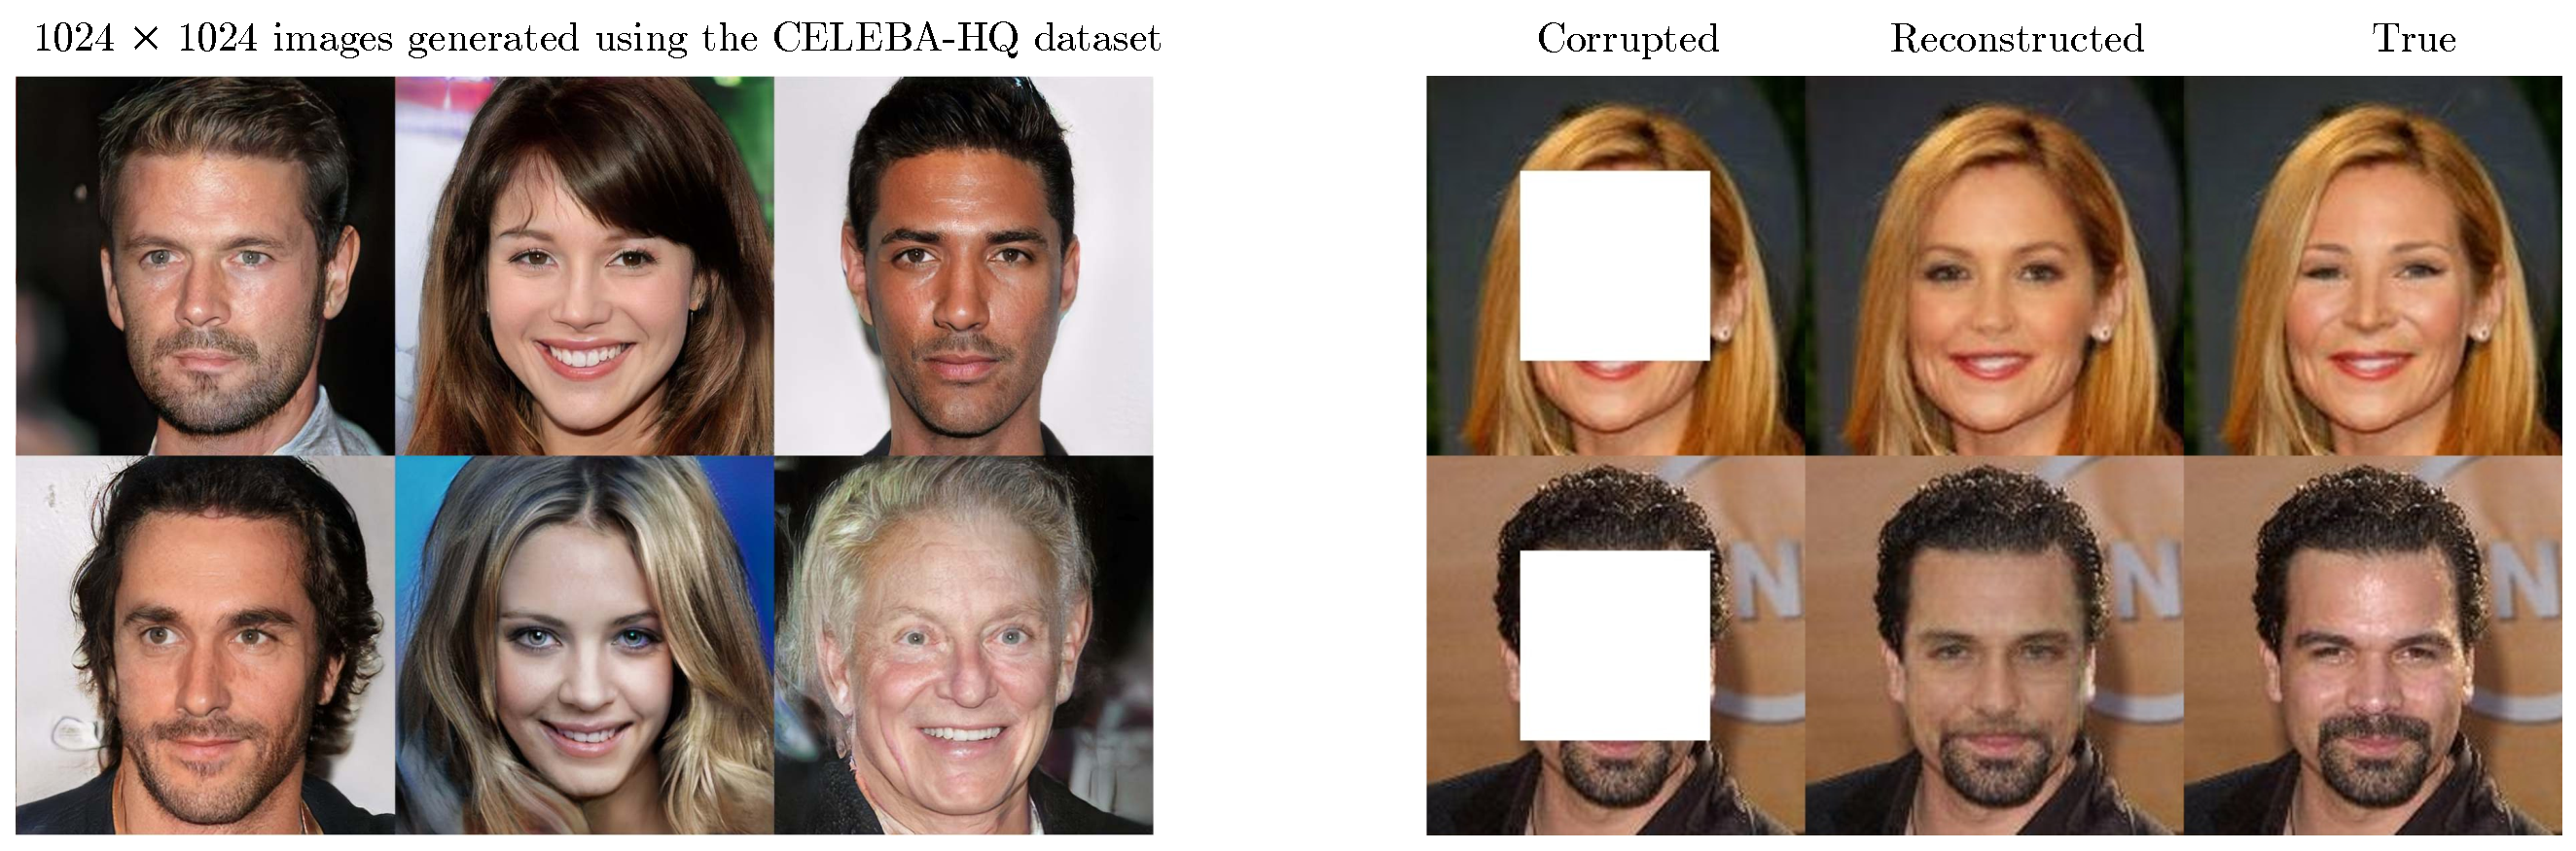
\includegraphics[width=\textwidth]{../figures/output.pdf}
\end{figure}
\end{center}
\end{frame}

\begin{frame}{Introduction}
Main ideas~\footnote{{\tiny \color{blue} Subhadip Mukherjee, Sören Dittmer, Zakhar Shumaylov, Sebastian Lunz, Ozan Öktem, Carola-Bibiane Schönlieb ``Learned Convex Regularizers for Inverse Problems", arxiv 2021}}:
\begin{itemize}
  \item Use deep learning to solve inverse problems
  \item With adaptation: {\bf enforce convexity on the learned regularizer} 
  \item Be pragmatic: lack of large amount of paired data
\end{itemize}
\vspace{1cm}
More motivation:
\begin{itemize}
\item Can show some convergence guarantees 
\item Design provable reconstruction algorithms
\item This is still less explored and poorly understood
\end{itemize}
\end{frame}

\begin{frame}{Inverse Problems in Computed Tomography}
\begin{itemize}
\item Estimate model parameters $\pmb{x}^{*} \in \mathbb{X}$ from data
$$
\pmb{y} = \mathcal{A}(\pmb{x}^{*}) + \pmb{e} \in \mathbb{Y}
$$
\item Forward operator $\mathcal{A}: \mathbb{X} \rightarrow Y$
\item $\mathbb{X}, \mathbb{Y}$ Hilbert spaces (after discretization, $\mathbb{X} = \mathbb{R}^{n}$ and $\mathbb{Y} = \mathbb{R}^{m}$)
\end{itemize}
\begin{block}{Variational Reconstruction}
$$
\min\limits_{\pmb{x} \in \mathbb{X}} \mathcal{L}_{\mathbb{Y}}\left( 
\mathcal{A}(\pmb{x}), \pmb{y}\right) + \lambda \mathcal{R}(\pmb{x})
$$
\end{block}
Where:
\begin{itemize}
\item $\mathcal{L}_{\mathbb{Y}}: \mathbb{Y} \times \mathbb{Y} \rightarrow \mathbb{R}$ measures data fidelity
\item $\mathcal{R}: \mathbb{X} \rightarrow \mathbb{R}$ penalizes undesirable solutions
\end{itemize}

\end{frame}

\begin{frame}{Classical Reconstruction Methods}
\begin{itemize}
\item Image-size: 160 x 160, angles: 40 (20), degrees: 0 - 180 (90)~\footnote{{\tiny \color{blue} https://github.com/markolalovic/learned-convex-regularizers}}
\item TV promotes sparsity in the image gradient: $\mathcal{R}(\pmb{x}) = \norm{\nabla \pmb{x}}_{1}$
\end{itemize}
\begin{center}
\begin{figure}
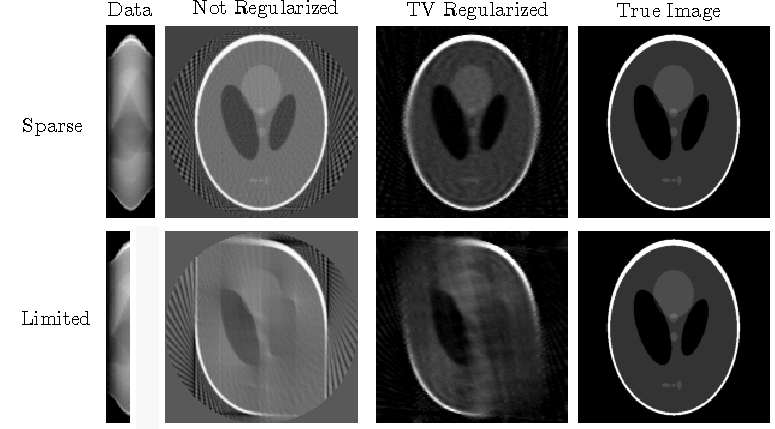
\includegraphics[width=.91\textwidth]{../figures/methods-annotated-crop.pdf}
\end{figure}
\end{center}
\end{frame}

\begin{frame}{Statistical Bayesian Formulation}
\begin{itemize}
\item $\pmb{x}^{*}$ and $\pmb{y}$ are modeled as realizations of $X$ and $Y$, which are $\mathbb{X}$- and $\mathbb{Y}$-valued random variables, respectively and
$$
Y = \mathcal{A}(X) + \pmb{e}
$$
\item Data likelihood: $\pi_{Y | X} (Y = y | X = \pmb{x}^{*}) = \pi_{\text{noise}}\left(\pmb{y} - \mathcal{A}(\pmb{x}^{*})\right)$
\item Prior: $\pi_{X}(\pmb{x})$
\item Posterior distribution: 
$$\pi_{X | Y}(\pmb{x} | \pmb{y}) = \frac{\pi_{Y | X}(\pmb{y} | \pmb{x}) \, \pi_{X}(\pmb{x})}{Z(y)}$$
\end{itemize}
\end{frame}

\begin{frame}{Supervised Learning}
\begin{itemize}
\item Training data: i.i.d.\ samples $\lbrace \pmb{x}_i, \pmb{y}_i \rbrace_{i=1}^{N}$ from the joint distribution $\pi_{X, Y}$
\item Parametric reconstruction operator: $G_{\theta}: \mathbb{Y} \rightarrow \mathbb{X}$, $\theta \in \Theta$
\item Loss function: $\mathcal{L}_{\mathbb{X}}: \mathbb{X} \times \mathbb{X} \rightarrow \mathbb{R}_{+}$
\item Risk minimization: $\min\limits_{\theta \in \Theta} \EX_{\pi_{X, Y}} \left[ \mathcal{L}_{\mathbb{X}}(X, \mathcal{G}_{\theta}(Y)) \right]$
\item Empirical risk minimization: $\min\limits_{\theta \in \Theta} \sum\limits_{i=1}^{N} \mathcal{L}_{\mathbb{X}}(x_i, \mathcal{G}_{\theta}(y_i))$
\item Example: 
\begin{itemize}
\item Using 0-1 loss and computing the mode, leads to so-called {\it maximum a-posterior probability} (MAP) estimate
\item Using Gibbs-type prior $\pi_{X}(\pmb{x}) \propto \exp{ \left(- \lambda \mathcal{R}(\pmb{x})\right)}$ is equivalent to classical variational reconstruction framework.
\end{itemize}
\end{itemize}
\end{frame}

\begin{frame}{Unsupervised Learning}
\begin{block}{Proposed Approach}
Keep the variational framework and only try to learn a suitable regularizer from the training data
\end{block}
Where:
\begin{itemize}
\item Training data: i.i.d.\ samples $\lbrace \pmb{x}_i \rbrace_{i = 1}^{N_{X}}$ from $\pi_{X}$ and $\lbrace \pmb{y}_i \rbrace_{i = 1}^{N_{Y}}$ from $\pi_{Y}$
\item Empirical risk minimization approach cannot be applied
\item Statistical characterization is an open problem
\end{itemize}
\end{frame}

\begin{frame}{Adversarial Learning}
We want to:
\begin{itemize}
\item Train regularization functional 
\item To suppress characteristic artifacts in the reconstruction
\item Because of the ill-posedness of the forward operator
\end{itemize}

\vspace{1cm}

How to do this:
\begin{itemize}
\item Minimize distributional distance between:
\begin{itemize}
\item True images, for example by using phantom images
\item Naive reconstructions, by using the pseudo-inverse on the data
\end{itemize}
\end{itemize}
\end{frame}

\begin{frame}{Wasserstein Distance}
\begin{itemize}
\item The Wasserstein-1 distance between two distributions $\mathbb{P}_{1}$ and $\mathbb{P}_{2}$
$$
\text{Wass}(\mathbb{P}_{1}, \mathbb{P}_{2}) := \inf_{\gamma \in \Pi(\mathbb{P}_{1}, \mathbb{P}_{2})} \norm{x_1 - x_2} d \gamma (x_1, x_2)
$$
\end{itemize}
\begin{center}
\begin{figure}
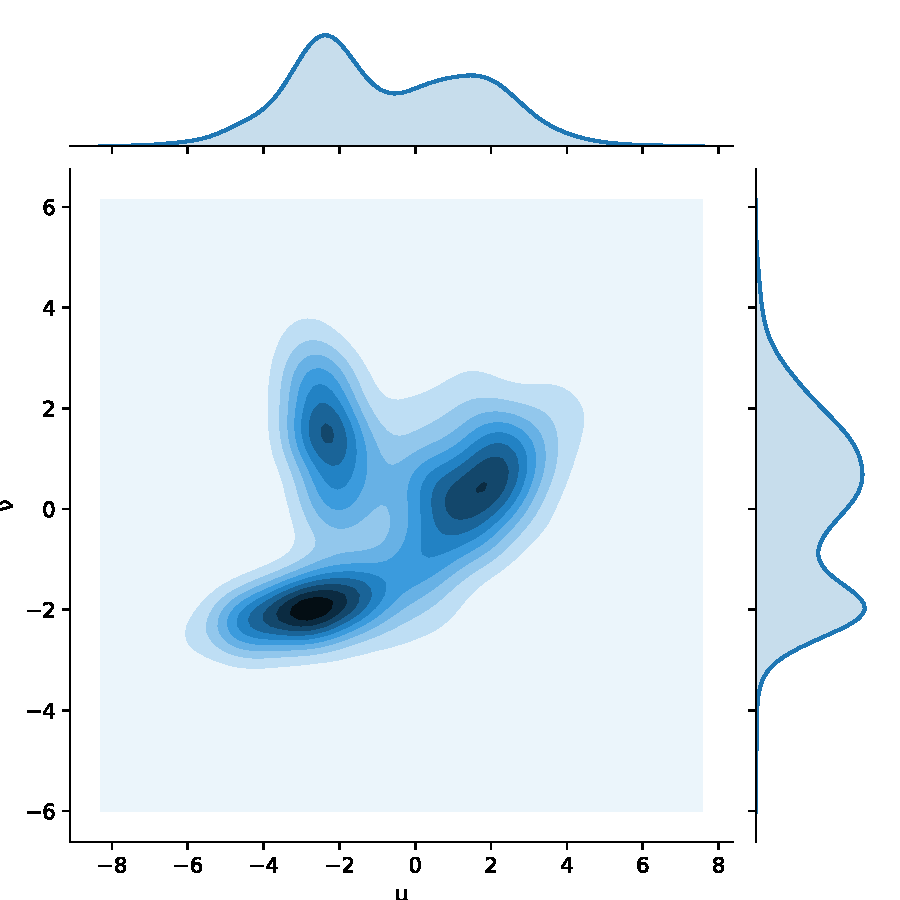
\includegraphics[width=.4\textwidth]{../figures/transport-plan.pdf}
\end{figure}
Minimal path length to transport mass $\mathbb{P}_1$ to $\mathbb{P}_2$~\footnote{{\tiny \color{blue} (By Lambdabadger licensed under CC BY-SA 4.0)}}
\end{center}
\end{frame}

\begin{frame}{Adversarial Regularizer}
\begin{itemize}
\item Variational reconstruction: $\min\limits_{x \in \mathbb{X}} \norm{\mathcal{A}(\pmb{x}) - \pmb{y}}_{2}^{2} + \lambda \mathcal{R}_{\theta}(\pmb{x})$
\item Two-step sequential approach:
\begin{itemize}
\item Learning:
\begin{align*}
\theta^{*} &= \argmin_{\theta} \EX_{\pi_{X}} \left[ \mathcal{R}_{\theta}(X) \right] - 
\EX_{\mathcal{A}_{\text{\#}}^{\dagger}\pi_{Y}} \left[ \mathcal{R}_{\theta}(X) \right] \\[.5em]
&\quad\text{ subject to } \mathcal{R}_{\theta} \in \text{1 - Lipschitz}
\end{align*}
\item Reconstruction: $\hat{x} = \argmin\limits_{\pmb{x} \in \mathbb{X}} \norm{\mathcal{A}(\pmb{x}) - \pmb{y}}_{2}^{2} + \lambda \mathcal{R}_{\theta^{*}}(\pmb{x})$
\end{itemize}
\item The 1-Lipschitz constraint is enforced by adding a gradient-penalty term
$$
\lambda_{gp} \EX_{\pi_{X^{(\epsilon)}}}\left[
\left( \norm{\nabla R_{\theta}\left( X^{(\epsilon)} \right) }_{2} - 1 \right)^{2}
\right]
$$
\item $X^{(\epsilon)}$ is uniformly sampled on the line-segment between $X$ and $\mathcal{A}^{\dagger}Y$
\end{itemize}
\end{frame}

\begin{frame}{Importance of 1-Lipschitz Constraint}
\begin{itemize}
\item View $\mathcal{R}_{\theta}$ as a classifier that learns to discriminate $\pi_{X}$ from $\pi_{\mathcal{\mathcal{A}_{\text{\#}}^{\dagger}} \pi_{Y}}$
\item Suppose the variational problem is solved via gradient-descent, starting with $\pmb{x}_{0}$ such that $\nabla_{\pmb{x}} \left( \norm{\mathcal{A}(\pmb{x} - \pmb{y}}_{2}^{2} \right)_{\pmb{x} = \pmb{x}_0} = 0$
\item $x_{0}$ is a sample from $\pi_{\mathcal{\mathcal{A}_{\text{\#}}^{\dagger}} \pi_{Y}}$ so $\mathcal{R}_{\theta}(\pmb{x}_{0})$ is large
\item $\pmb{x} = \pmb{x}_0 - \eta \nabla \mathcal{R}_{\theta}(\pmb{x}_0)$
\item The output of $\mathcal{R}_{\theta}$ does not change much going from $\pmb{x}_0$ to $\pmb{x}_1$
$$
|\mathcal{R}_{\theta}(\pmb{x}_1) - \mathcal{R}_{\theta}(\pmb{x}_0)|
\leq \norm{\pmb{x}_1 - \pmb{x}_0} = \eta \norm{\nabla \mathcal{R}_{\theta}(\pmb{x}_0}_{2} 
\leq \eta
$$
\item Preventing learning sharp boundaries
\end{itemize}
\end{frame}

\begin{frame}{Adversarial Convex Regularizer}
\begin{itemize}
\item Let $\mathcal{R}_{\theta}(\pmb{x}) = \mathcal{R}_{\theta}'(\pmb{x}) + \rho_0 \norm{x}^{2}_{2}$ where $\mathcal{R}_{\theta}'$ is convex and Lipschitz
\end{itemize}
\centering
\vspace{.5cm}
{\bf Results:}
\begin{itemize}
\item Existence and uniqueness: follow by strong-convexity
\item Stability: $\hat{x}_{\lambda}(y)$ is continuous in $y$, in particular ($\mathcal{A}$ is assumed to be linear and bounded, $\beta_1$ is the operator norm)
$$
\norm{\hat{x}_{\lambda}(y^{\delta_1}) - \hat{x}_{\lambda}(y)}_{2} \leq
\frac{\beta_1 \delta_1}{\lambda \rho_0}
\qquad \text{ if } \quad \norm{y^{\delta_1} - y}_{2} \leq \delta_1
$$
\item Convergence: $\hat{x}_{\lambda}(y) \rightarrow x^{\dagger}$ if $\lambda \rightarrow 0$ and $\frac{\delta}{\lambda} \rightarrow 0$ when $\delta = \norm{\pmb{e}}_{2} \rightarrow 0$, where
$$
x^{\dagger} = \argmin\limits_{x \in \mathbb{X}} \mathcal{R}_{\theta}
\qquad \text{subject to} \quad \mathcal{A}(x) = y^{0}
$$
\item Implies existence of convergent sub-gradient algorithm
\end{itemize}
\end{frame}

\begin{frame}{Adversarial Convex Regularizer - Architecture}
From convex theory:
\begin{itemize}
\item Let $f_i: \mathbb{R} \rightarrow \mathbb{R}$ be convex, then so is
$\sum_{i} \beta_i f_i $ for $\beta_i \geq 0$
\item Let $f_1, f_2: \mathbb{R} \rightarrow \mathbb{R}$ be convex, $f_1(x) \leq f_1(y)$ whenever $x \leq y$ $\implies$ $f_1 \circ f_2$ is convex:
\end{itemize}
\begin{align*}
f_2(\lambda x_1 + (1-\lambda)x_2) &\leq 
\lambda f_2(x_1) + (1-\lambda)f(x_2) \\[.5em]
\implies (f_1 \circ f_2) (\lambda x_1 + (1-\lambda)x_2) &\leq 
f_1(\lambda f_2(x_1) + (1 - \lambda)f_2(x_2))  \\[.5em]
&\leq \lambda \, (f_1 \circ f_2) (x_1) + (1 - \lambda) (f_1 \circ f_2)(x_2)
\end{align*}
Input Convex Neural Network (ICNN):
\begin{itemize}
\item $z^{(1)}(\pmb{x}) = \phi \left( W_{x}^{(1)}x + b^{(1)}  \right)$ 
\item $\phi$ acts component-wise such as Rectified Linear Unit (ReLU) $x \mapsto \max(0, x)$ is convex and monotonically non-decreasing
\end{itemize}
\end{frame}

\begin{frame}{Adversarial Convex Regularizer - Architecture Contd.}
\begin{itemize}
\item $z^{(2)}(\pmb{x}) = \phi \left( W_{z}^{(1)}z^{(1)}(x) + W_{x}^{(2)}x + b^{(2)}  \right)$, $W_{z}^{(1)} \geq 0$, is convex in $x$
\item $z^{(i+1)}(\pmb{x}) = \phi \left( W_{z}^{(i)}z^{(i)}(x) + W_{x}^{(i+1)}x + b^{(i+1)}  \right)$, $i = 1, 2, \dots, L = 10$
\item $\mathcal{R}_{\theta} = \sum_{j} z_{j}^{(L+1)}(x) + \rho_{0}' \sum_{k=1}^{M} \norm{U^{(k)}x}_{1} + \rho_{0} \norm{x}_{2}^{2}$
\item $\sum_{j} z_{j}^{(L+1)}(x)$ is convex and filter-bank term is convex, norms are penalized to impose 1-Lipschitz condition
\item The squared $\ell_{2}$ term makes the regularizer strongly-convex
\end{itemize}
\begin{center}
\begin{figure}
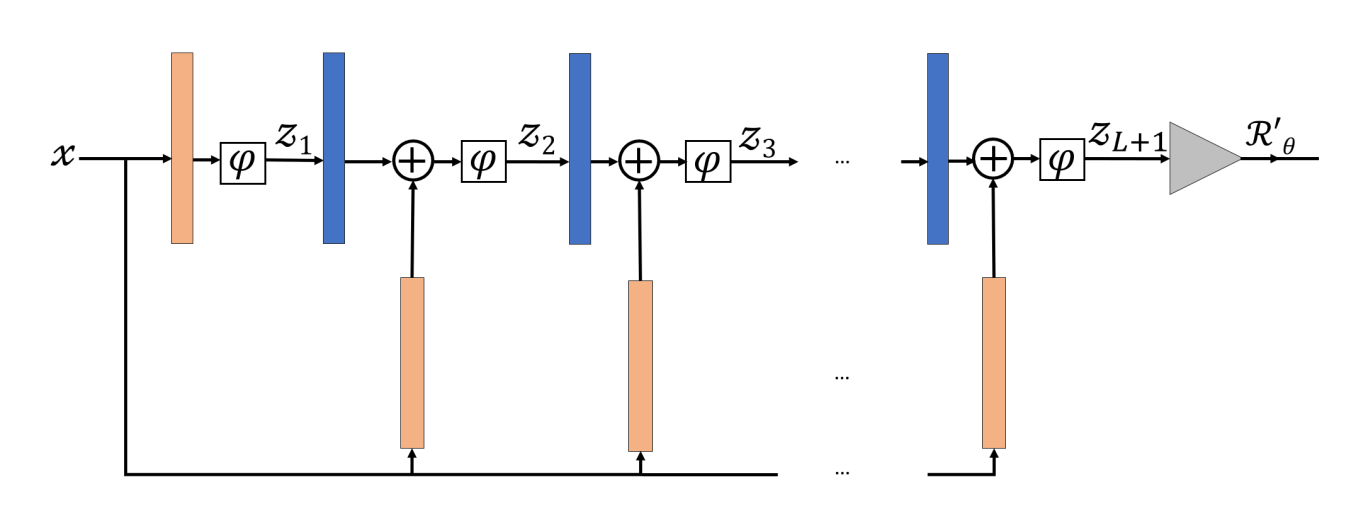
\includegraphics[width=.6\textwidth]{../figures/arhitecture.png}
\end{figure}
\end{center}
\end{frame}

\begin{frame}{Convergence of sub-gradient method}
\begin{itemize}
\item We have objective functional of the form:
$$
J(\pmb{x}) = \underbrace{\norm{\mathcal{A}(\pmb{x}) - \pmb{y}}_{2}^{2} + \lambda \rho_0 \norm{\pmb{x}}_{2}^{2}}_\text{$f(\pmb{x})$ smooth, strongly-convex} \quad
+ \underbrace{\lambda \mathcal{R}_{\theta}'(\pmb{x})}_\text{g(\pmb{x}) convex, Lipschitz}
$$
\item The sub-gradient method 
$$
x_{k+1} = x_{k} - \eta_{k} \left(\nabla f(x_k) + u_k\right) 
\quad \text{where} \quad u_k \in \partial g(x_k)
$$
\item Converges: 
\begin{itemize}
\item Let $e_{k} = \norm{x_k - \hat{x}}_{2}^{2}$, derive the inequality $e_{k+1} \leq e_{k} - \text{Quant.}(\lambda, \rho_0, L_{\nabla})$, if
$$
\eta_{k} = \lambda \rho_{0} \frac{\norm{x_{k} - \hat{x}}_{2}^{2}}{\norm{\nabla f(x_{k}) + u_{k}}_{2}^{2}}
$$
\item Take the limit on both sides, limit exists by monotonicity and boundedness from below
\end{itemize}
\end{itemize}
\end{frame}

\begin{frame}{Limited-Angle CT Results}
  \begin{center}
    \begin{figure}
      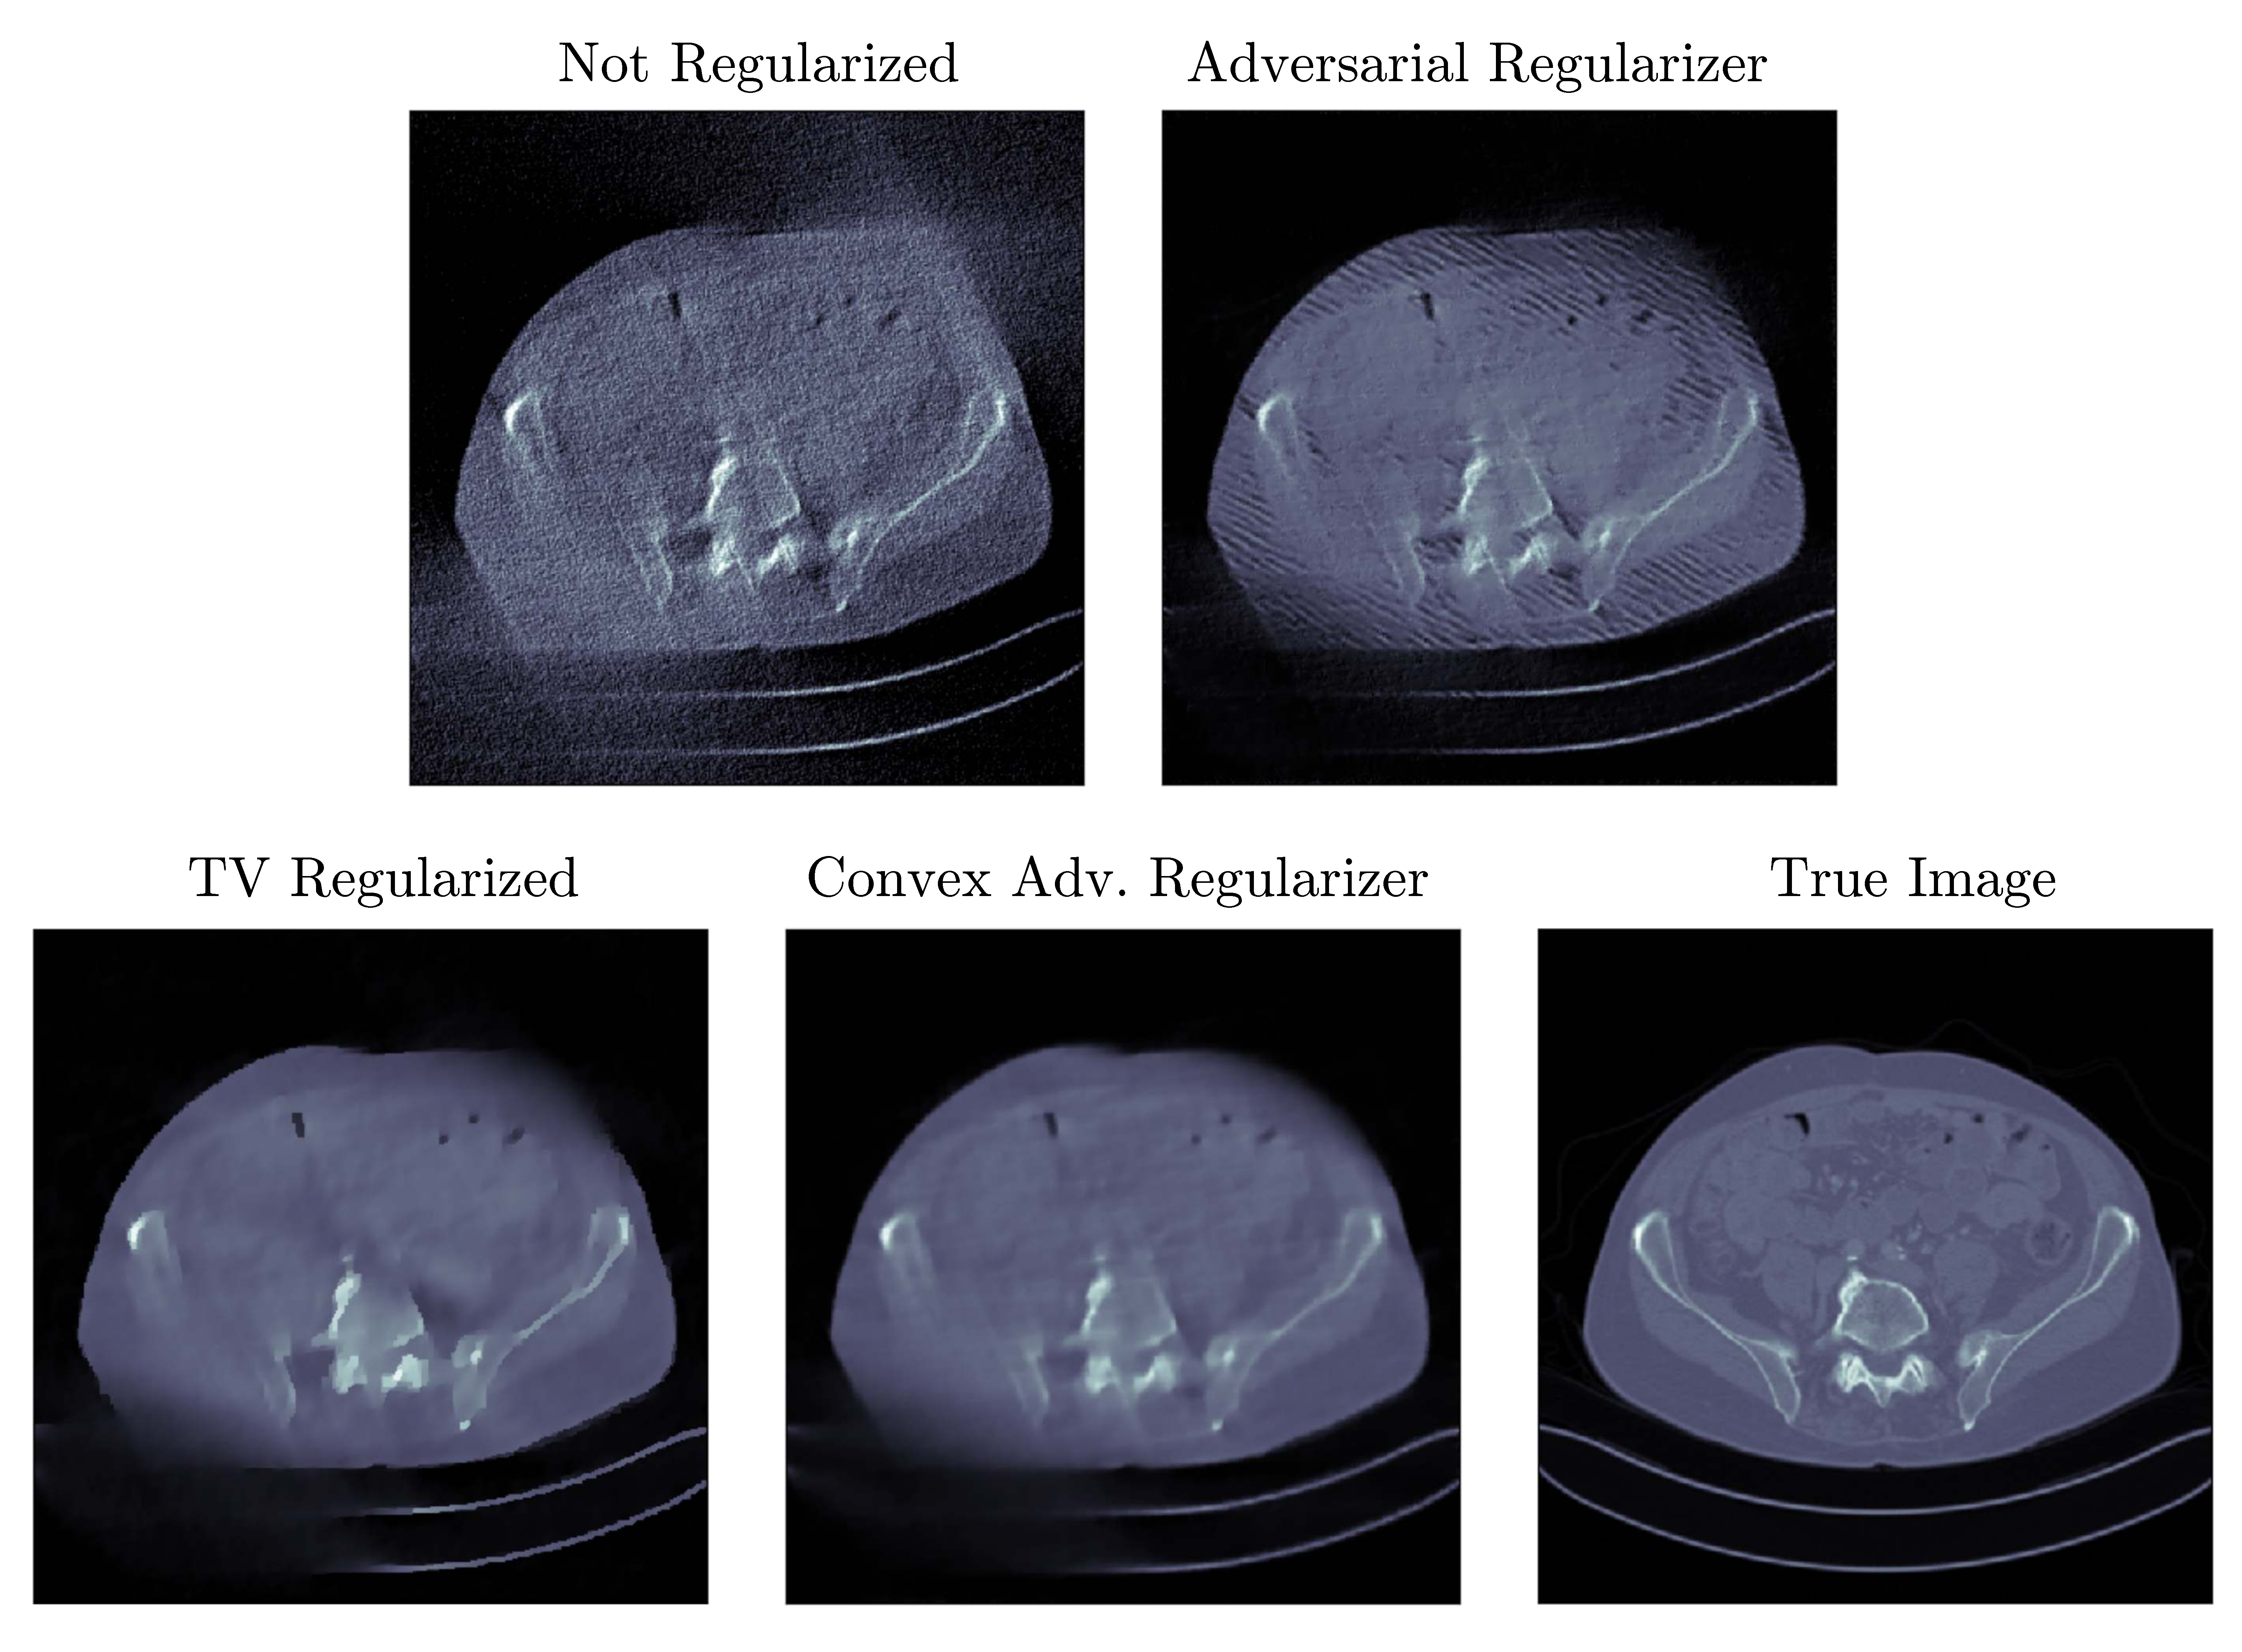
\includegraphics[width=.9\textwidth]{../figures/results-final.pdf}
    \end{figure}
  \end{center}
\end{frame}

\begin{frame}{Open Questions}
\begin{itemize}
\item Convex regularizers often underestimate the high-amplitude components of the true image
\item The convexity does not seem to be a significant restriction
\item There are 23 citations according to Google:
\end{itemize}
\begin{center}
\begin{figure}
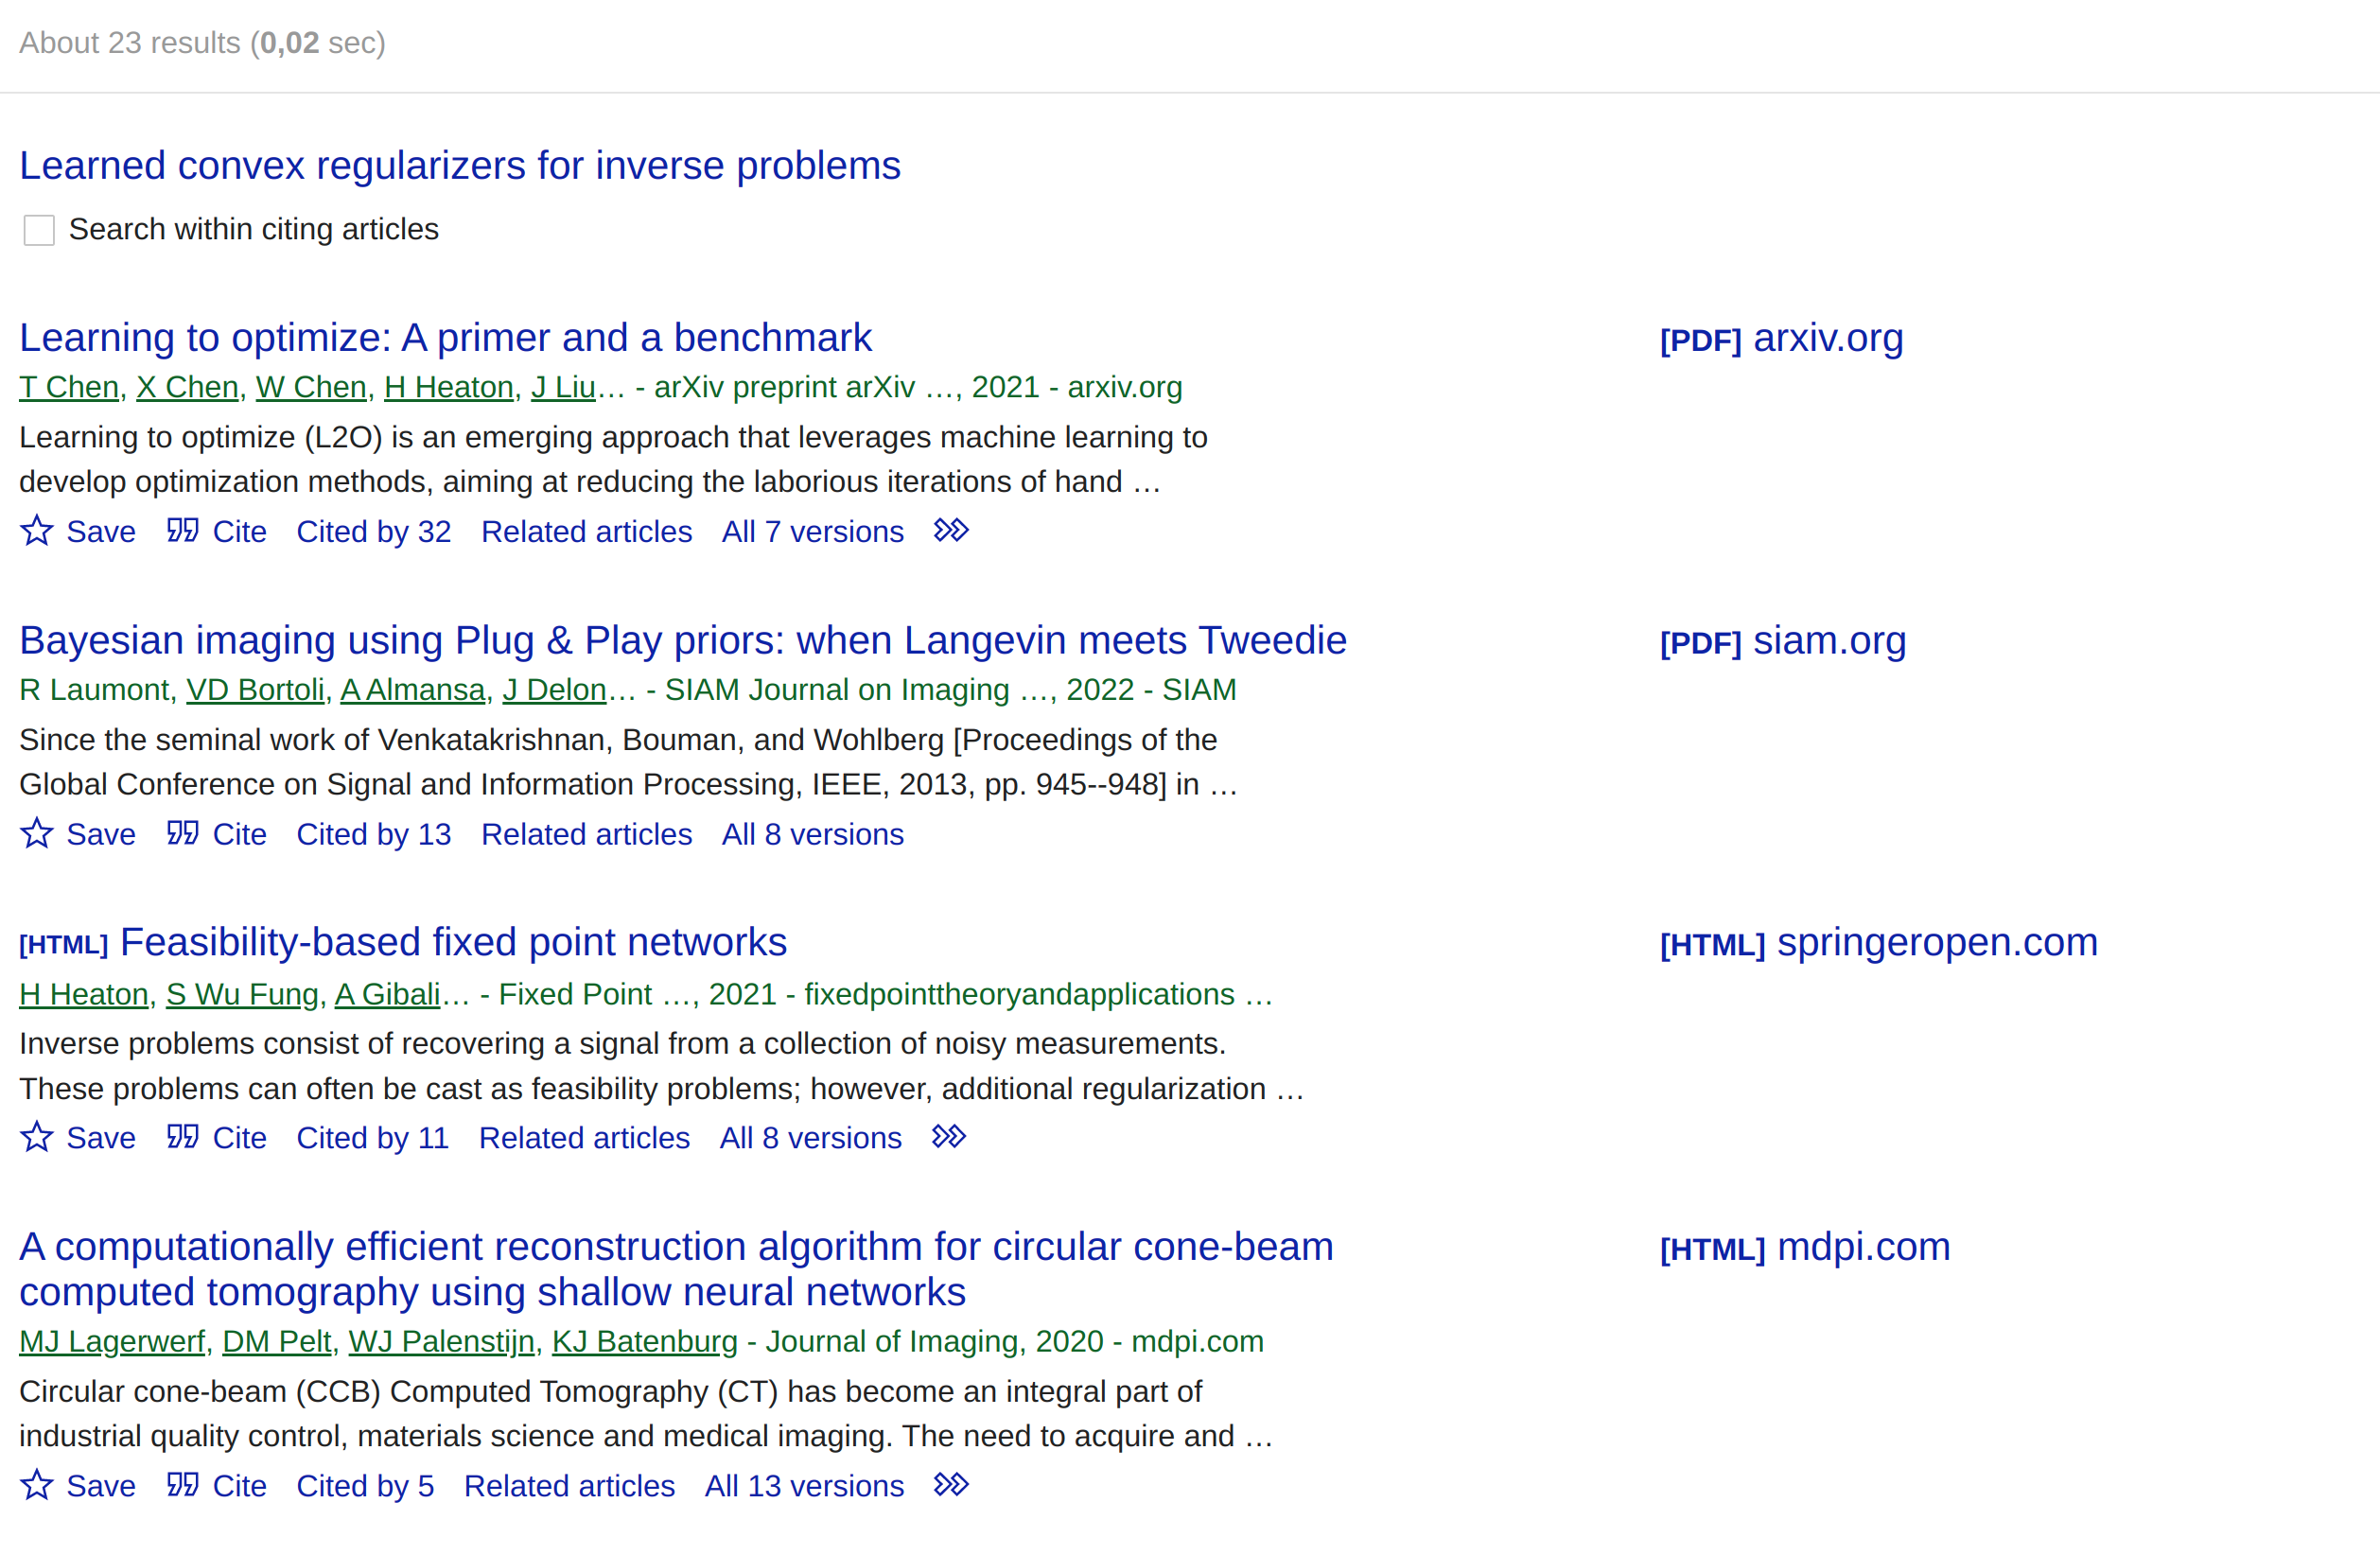
\includegraphics[width=.7\textwidth]{../figures/citations.png}
\end{figure}
\end{center}
\end{frame}

\begin{frame}{Wasserstein Distance - Justification}
\begin{itemize}
\item The Kantorovich duality allows to equivalently characterize via 
$$
\text{Wass}(\mathbb{P}_{n}, \mathbb{P}_{r}) := \sup_{f \in 1-\text{Lip}} \varepsilon_{U \sim \mathbb{P}_{n}} f(U) - \varepsilon_{U \sim \mathbb{P}_{r}} f(U)
$$
\item Denote now by $f^{*}$ an optimizer of the dual formulation of the Wasserstein distance
\end{itemize}
\end{frame}

\begin{frame}{Assumptions}
\begin{itemize}
\item Data Manifold Assumption (DMA): The measure $\mathbb{P}_{r}$ is supported on a weakly compact set $\mathcal{M}$
\item Denote by $P_{\mathcal{M}}: D \rightarrow \mathcal{M}$, $u \mapsto \argmin_{v \in \mathcal{M}} \norm{u - v}$ the projection onto the data manifold
\item Projection Assumption: $(P_{\mathcal{M}})_{\text{\#}}(\mathbb{P}_{n}) = \mathbb{P}_r$
\item Corresponds to a low-noise assumption - noise level low in comparison to manifold curvature
\end{itemize}
\end{frame}

\begin{frame}{Manifold Lemma}
\begin{block}{Theorem}
Assume DMA and low-noise assumption. Then the distance function to the data manifold
$$
u \mapsto \min\limits_{v \in \mathcal{M}} \norm{u - v}_{2}
$$
is a maximizer to the Wasserstein Loss
$$
\sup_{f \in 1-\text{Lip}} \EX_{U \sim \mathbb{P}_{n}} f(U) 
- \EX_{U \sim \mathbb{P}_{r}} f(U)
$$
\end{block}
\end{frame}

\begin{frame}{Approximating $f^{*}$}
Idea from Wasserstein Generative Adversarial Networks (WGANs)
\begin{itemize}
\item Use a neural network (critic) to approximate $f^{*}$
\item Train the network with the loss
$$
\EX_{U \sim \mathcal{P}_{r}}[\Psi_{Theta}(U)] - 
\EX_{U \sim \mathcal{P}_{n}}[\Psi_{Theta}(U)] +
\mu \cdot \EX\left[ \left( 
\norm{\nabla_{u} \Psi_{\Theta}(U)}_{*} - 1
\right)^{2}_{+}
\right]
$$
\item 1-Lipschitz constraint into penalty term (WGAN-GP)
\end{itemize}
\end{frame}

\end{document}